%%%%%%%%%%%%%%%%%%%%%%%%%%%%%%%%%%%%%%%%%%%%%%%%%%%%%%%%%%%%%%%%%%%%%%%%%%%%%%%%%%%%%%%%%%%%%%%%%%%%%%%%%%%%%%%%%%%%%%%%%%%%%%%%%%%%%%%%%%%%%%%%%%%%%%%%%%%%%%%%%%%
% Written By Michael Brodskiy
% Class: Fundamentals of Electronics
% Professor: I. Salama
%%%%%%%%%%%%%%%%%%%%%%%%%%%%%%%%%%%%%%%%%%%%%%%%%%%%%%%%%%%%%%%%%%%%%%%%%%%%%%%%%%%%%%%%%%%%%%%%%%%%%%%%%%%%%%%%%%%%%%%%%%%%%%%%%%%%%%%%%%%%%%%%%%%%%%%%%%%%%%%%%%%

\include{Includes.tex}

\title{Pre-Lab 3}
\date{October 28, 2024}
\author{Michael Brodskiy\\ \small Professor: M. Onabajo}

\begin{document}

\maketitle

\begin{enumerate}

  \item We may begin by finding a DC equivalent circuit (capacitors become open circuits):

    \begin{figure}[H]
      \centering
      \tikzset{every picture/.style={line width=0.75pt}} %set default line width to 0.75pt        

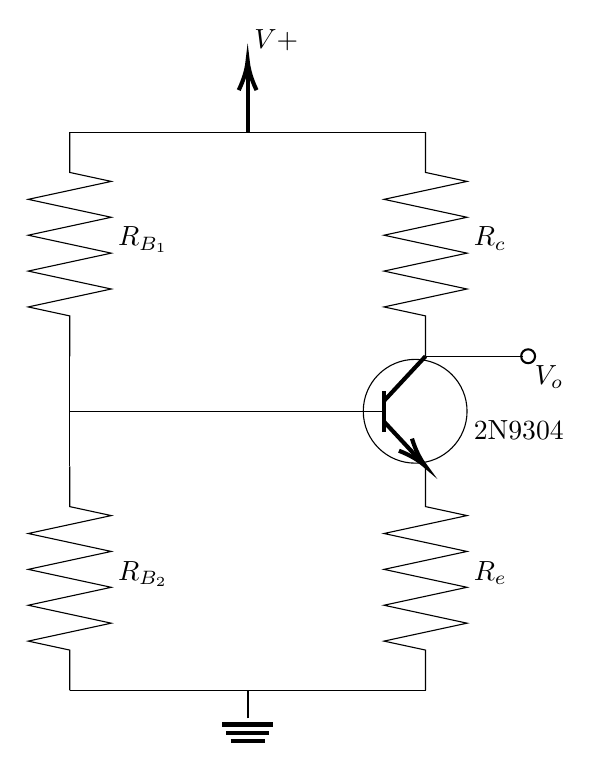
\begin{tikzpicture}[x=0.75pt,y=0.75pt,yscale=-1,xscale=1]
%uncomment if require: \path (0,497); %set diagram left start at 0, and has height of 497

%Shape: Resistor [id:dp08557489822351128] 
\draw   (140,71) -- (140,90.44) -- (160,94.76) -- (120,103.4) -- (160,112.04) -- (120,120.68) -- (160,129.32) -- (120,137.96) -- (160,146.6) -- (120,155.24) -- (140,159.56) -- (140,179) ;
%Shape: Resistor [id:dp5471354453834067] 
\draw   (140,232) -- (140,251.44) -- (160,255.76) -- (120,264.4) -- (160,273.04) -- (120,281.68) -- (160,290.32) -- (120,298.96) -- (160,307.6) -- (120,316.24) -- (140,320.56) -- (140,340) ;
%Straight Lines [id:da10613850567534644] 
\draw    (281.42,205.5) -- (140,205.5) ;
%Shape: Resistor [id:dp42863709400980965] 
\draw   (311.42,71) -- (311.42,90.44) -- (331.42,94.76) -- (291.42,103.4) -- (331.42,112.04) -- (291.42,120.68) -- (331.42,129.32) -- (291.42,137.96) -- (331.42,146.6) -- (291.42,155.24) -- (311.42,159.56) -- (311.42,179) ;
%Shape: Resistor [id:dp18218903209345216] 
\draw   (311.42,232) -- (311.42,251.44) -- (331.42,255.76) -- (291.42,264.4) -- (331.42,273.04) -- (291.42,281.68) -- (331.42,290.32) -- (291.42,298.96) -- (331.42,307.6) -- (291.42,316.24) -- (311.42,320.56) -- (311.42,340) ;
%Straight Lines [id:da236864146953923] 
\draw    (140,179) -- (140,232) ;
%Shape: Circle [id:dp6263492261348075] 
\draw   (281.42,205.5) .. controls (281.42,191.69) and (292.61,180.5) .. (306.42,180.5) .. controls (320.23,180.5) and (331.42,191.69) .. (331.42,205.5) .. controls (331.42,219.31) and (320.23,230.5) .. (306.42,230.5) .. controls (292.61,230.5) and (281.42,219.31) .. (281.42,205.5) -- cycle ;
%Straight Lines [id:da5434466420085665] 
\draw    (291.42,205.5) -- (281.42,205.5) ;
%Straight Lines [id:da8222789328378522] 
\draw [line width=1.5]    (291.42,215.5) -- (291.42,195.5) ;
%Straight Lines [id:da6868248647799469] 
\draw [line width=1.5]    (291.42,210.5) -- (309.38,229.8) ;
\draw [shift={(311.42,232)}, rotate = 227.07] [color={rgb, 255:red, 0; green, 0; blue, 0 }  ][line width=1.5]    (14.21,-4.28) .. controls (9.04,-1.82) and (4.3,-0.39) .. (0,0) .. controls (4.3,0.39) and (9.04,1.82) .. (14.21,4.28)   ;
%Straight Lines [id:da7170401481045089] 
\draw [line width=1.5]    (311.42,179) -- (291.42,200.5) ;
%Straight Lines [id:da09379764529365986] 
\draw    (311.42,340) -- (140,340) ;
%Straight Lines [id:da37329225941611255] 
\draw    (311.42,71) -- (140,71) ;
%Straight Lines [id:da20374241030260287] 
\draw [line width=1.5]    (225.71,71) -- (225.71,39.58) ;
\draw [shift={(225.71,36.58)}, rotate = 90] [color={rgb, 255:red, 0; green, 0; blue, 0 }  ][line width=1.5]    (14.21,-4.28) .. controls (9.04,-1.82) and (4.3,-0.39) .. (0,0) .. controls (4.3,0.39) and (9.04,1.82) .. (14.21,4.28)   ;
%Straight Lines [id:da7615603326736993] 
\draw    (358.49,179) -- (311.42,179) ;
\draw [shift={(360.84,179)}, rotate = 180] [color={rgb, 255:red, 0; green, 0; blue, 0 }  ][line width=0.75]      (0, 0) circle [x radius= 3.35, y radius= 3.35]   ;
%Straight Lines [id:da09982064594930351] 
\draw [line width=0.75]    (225.71,353.42) -- (225.71,340) ;
%Straight Lines [id:da7825511264162391] 
\draw [line width=1.5]    (213.5,356.42) -- (237.92,356.42) ;
%Straight Lines [id:da8263231613187413] 
\draw [line width=1.5]    (215.5,360.42) -- (235.92,360.42) ;
%Straight Lines [id:da4438946372208784] 
\draw [line width=1.5]    (217.5,364.42) -- (233.92,364.42) ;

% Text Node
\draw (227.71,33.18) node [anchor=south west] [inner sep=0.75pt]    {$V+$};
% Text Node
\draw (362.84,182.4) node [anchor=north west][inner sep=0.75pt]    {$V_{o}$};
% Text Node
\draw (333.42,208.5) node [anchor=north west][inner sep=0.75pt]   [align=left] {2N9304};
% Text Node
\draw (333.42,115.44) node [anchor=north west][inner sep=0.75pt]    {$R_{c}$};
% Text Node
\draw (333.42,276.44) node [anchor=north west][inner sep=0.75pt]    {$R_{e}$};
% Text Node
\draw (162,115.44) node [anchor=north west][inner sep=0.75pt]    {$R_{B_{1}}$};
% Text Node
\draw (162,276.44) node [anchor=north west][inner sep=0.75pt]    {$R_{B_{2}}$};


\end{tikzpicture}

      \caption{DC-Equivalent Circuit}
      \label{fig:1}
    \end{figure}

    We then use a Th\'evenin equivalent at the voltage source:

    $$V_{Th}=V^+\left( \frac{10k}{47k+10k} \right)$$
    $$V_{Th}=1.7544[\si{\volt}]$$
    $$R_{Th}=\frac{(47)(10)}{47+10}[\si{\kilo\ohm}]$$
    $$R_{Th}=8.2456[\si{\kilo\ohm}]$$

    This gives us the following circuit:

    \begin{figure}[H]
      \centering
      \tikzset{every picture/.style={line width=0.75pt}} %set default line width to 0.75pt        

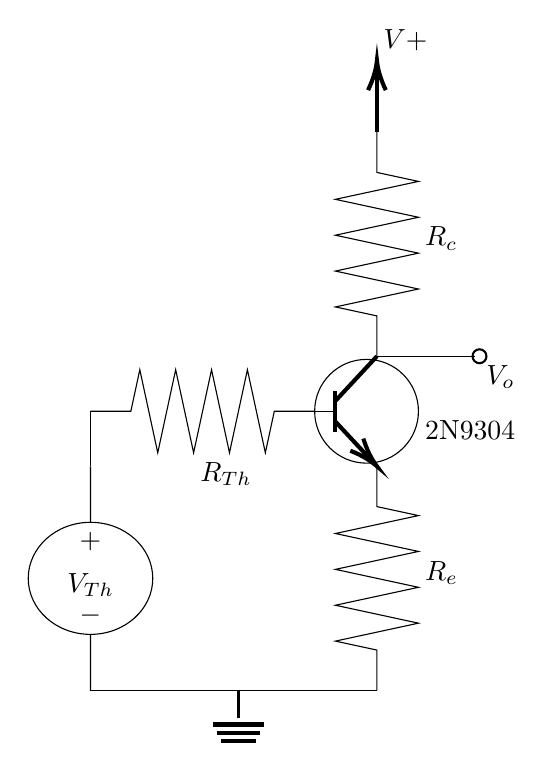
\begin{tikzpicture}[x=0.75pt,y=0.75pt,yscale=-1,xscale=1]
%uncomment if require: \path (0,497); %set diagram left start at 0, and has height of 497

%Shape: Resistor [id:dp5471354453834067] 
\draw   (173.42,205.5) -- (192.86,205.5) -- (197.18,185.5) -- (205.82,225.5) -- (214.46,185.5) -- (223.1,225.5) -- (231.74,185.5) -- (240.38,225.5) -- (249.02,185.5) -- (257.66,225.5) -- (261.98,205.5) -- (281.42,205.5) ;
%Shape: Resistor [id:dp42863709400980965] 
\draw   (311.42,71) -- (311.42,90.44) -- (331.42,94.76) -- (291.42,103.4) -- (331.42,112.04) -- (291.42,120.68) -- (331.42,129.32) -- (291.42,137.96) -- (331.42,146.6) -- (291.42,155.24) -- (311.42,159.56) -- (311.42,179) ;
%Shape: Resistor [id:dp18218903209345216] 
\draw   (311.42,232) -- (311.42,251.44) -- (331.42,255.76) -- (291.42,264.4) -- (331.42,273.04) -- (291.42,281.68) -- (331.42,290.32) -- (291.42,298.96) -- (331.42,307.6) -- (291.42,316.24) -- (311.42,320.56) -- (311.42,340) ;
%Straight Lines [id:da236864146953923] 
\draw    (173.42,205.5) -- (173.42,232) ;
%Shape: Circle [id:dp6263492261348075] 
\draw   (281.42,205.5) .. controls (281.42,191.69) and (292.61,180.5) .. (306.42,180.5) .. controls (320.23,180.5) and (331.42,191.69) .. (331.42,205.5) .. controls (331.42,219.31) and (320.23,230.5) .. (306.42,230.5) .. controls (292.61,230.5) and (281.42,219.31) .. (281.42,205.5) -- cycle ;
%Straight Lines [id:da5434466420085665] 
\draw    (291.42,205.5) -- (281.42,205.5) ;
%Straight Lines [id:da8222789328378522] 
\draw [line width=1.5]    (291.42,215.5) -- (291.42,195.5) ;
%Straight Lines [id:da6868248647799469] 
\draw [line width=1.5]    (291.42,210.5) -- (309.38,229.8) ;
\draw [shift={(311.42,232)}, rotate = 227.07] [color={rgb, 255:red, 0; green, 0; blue, 0 }  ][line width=1.5]    (14.21,-4.28) .. controls (9.04,-1.82) and (4.3,-0.39) .. (0,0) .. controls (4.3,0.39) and (9.04,1.82) .. (14.21,4.28)   ;
%Straight Lines [id:da7170401481045089] 
\draw [line width=1.5]    (311.42,179) -- (291.42,200.5) ;
%Straight Lines [id:da09379764529365986] 
\draw    (311.42,340) -- (173.42,340) ;
%Straight Lines [id:da20374241030260287] 
\draw [line width=1.5]    (311.42,71) -- (311.42,39.58) ;
\draw [shift={(311.42,36.58)}, rotate = 90] [color={rgb, 255:red, 0; green, 0; blue, 0 }  ][line width=1.5]    (14.21,-4.28) .. controls (9.04,-1.82) and (4.3,-0.39) .. (0,0) .. controls (4.3,0.39) and (9.04,1.82) .. (14.21,4.28)   ;
%Straight Lines [id:da7615603326736993] 
\draw    (358.49,179) -- (311.42,179) ;
\draw [shift={(360.84,179)}, rotate = 180] [color={rgb, 255:red, 0; green, 0; blue, 0 }  ][line width=0.75]      (0, 0) circle [x radius= 3.35, y radius= 3.35]   ;
%Straight Lines [id:da09982064594930351] 
\draw [line width=0.75]    (244.71,353.42) -- (244.71,340) ;
%Straight Lines [id:da7825511264162391] 
\draw [line width=1.5]    (232.5,356.42) -- (256.92,356.42) ;
%Straight Lines [id:da8263231613187413] 
\draw [line width=1.5]    (234.5,360.42) -- (254.92,360.42) ;
%Straight Lines [id:da4438946372208784] 
\draw [line width=1.5]    (236.5,364.42) -- (252.92,364.42) ;
%Shape: Output [id:dp833046385605702] 
\draw   (173.42,259) .. controls (189.99,259) and (203.42,271.09) .. (203.42,286) .. controls (203.42,300.91) and (189.99,313) .. (173.42,313) .. controls (156.85,313) and (143.42,300.91) .. (143.42,286) .. controls (143.42,271.09) and (156.85,259) .. (173.42,259) -- cycle (173.42,232) -- (173.42,259) (173.42,340) -- (173.42,313) ;

% Text Node
\draw (313.42,33.18) node [anchor=south west] [inner sep=0.75pt]    {$V+$};
% Text Node
\draw (362.84,182.4) node [anchor=north west][inner sep=0.75pt]    {$V_{o}$};
% Text Node
\draw (333.42,208.5) node [anchor=north west][inner sep=0.75pt]   [align=left] {2N9304};
% Text Node
\draw (333.42,115.44) node [anchor=north west][inner sep=0.75pt]    {$R_{c}$};
% Text Node
\draw (333.42,276.44) node [anchor=north west][inner sep=0.75pt]    {$R_{e}$};
% Text Node
\draw (225.1,228.9) node [anchor=north west][inner sep=0.75pt]    {$R_{Th}$};
% Text Node
\draw (173.42,262.4) node [anchor=north] [inner sep=0.75pt]    {$+$};
% Text Node
\draw (173.42,309.6) node [anchor=south] [inner sep=0.75pt]    {$-$};
% Text Node
\draw (173.49,289.19) node    {$V_{Th}$};


\end{tikzpicture}

      \caption{Th\'evenin Equivalent Circuit}
      \label{fig:2}
    \end{figure}

    From here, we see that $I_B$ flows through $R_{Th}$, $I_C$ flows through $R_C$, and $I_E$ flows through $R_E$. We may begin by writing the KVL for the loop:

    $$-V_{Th}+I_{B}R_{Th}+V_{BE}+I_ER_e=0$$

    Per our equations, we know that $I_E=(1+\beta)I_B$, so we substitute and rearrange to get:

    $$I_B=\frac{V_{Th}-V_{BE}}{R_{Th}+(1+\beta)R_e}$$

    We can then analyze the provided cases:

    \begin{itemize}

      \item $\beta=80$:

        $$I_B=\frac{1.7544-.7}{8.2456\cdot10^3+(1+80)(220)}$$
        $$\boxed{I_B\Big|_{\beta=80}=40.452[\si{\micro\ampere}]}$$

        $$I_C=80I_B$$
        $$\boxed{I_C=3.236[\si{\milli\ampere}]}$$

        $$V_C=V^+-I_CR_C$$
        $$V_C=10-(3.236)(1)$$
        $$\boxed{V_C=6.764[\si{\volt}]}$$

        $$V_B=V_{Th}-I_BR_{Th}$$
        $$V_B=1.7544-(40.452\cdot10^{-3})(8.2456)$$
        $$\boxed{V_B=1.7541[\si{\volt}]}$$

        Given that $V_C>V_B$, the collector-to-base junction is reverse-biased, meaning that the transistor is active. Thus, the Q-point is stable.

      \item $\beta=300$:

        $$I_B=\frac{1.7544-.7}{8.2456\cdot10^3+(1+300)(220)}$$
        $$\boxed{I_B\Big|_{\beta=300}=14.16[\si{\micro\ampere}]}$$

        $$I_C=300I_B$$
        $$\boxed{I_C=4.248[\si{\milli\ampere}]}$$

        $$V_C=V^+-I_CR_C$$
        $$V_C=10-(4.248)(1)$$
        $$\boxed{V_C=5.752[\si{\volt}]}$$

        $$V_B=V_{Th}-I_BR_{Th}$$
        $$V_B=1.7544-(14.16\cdot10^{-3})(8.2456)$$
        $$\boxed{V_B=1.6376[\si{\volt}]}$$

        Given that $V_C>V_B$, the collector-to-base junction is reverse-biased, meaning that the transistor is active. Thus, the Q-point is stable.

    \end{itemize}

    We may see that, since the transistor is active for both $\beta=80$ and $\beta=300$, the Q-point is stable. As such, the operating point is stable for such variation of $\beta$.

  \item Read through, no questions \textcolor{green}{\checkmark}

  \item We know that the amplifier will be of the form:

    \begin{figure}[H]
      \centering
      \include{Figures/PL4d3}
      \caption{Amplifier Design}
      \label{fig:3}
    \end{figure}

    We want to use the most extreme values so that the circuit can tolerate these. Furthermore, we know that the gain will be:

    $$A_v=-\frac{R_c}{R_e}$$
    $$R_c=21R_e$$

    Thus, let us take values such that:

    $$R_c=21[\si{\kilo\ohm}]\quad\text{ and }R_e=1[\si{\kilo\ohm}]$$

    From here, we want to make sure that the BJT remains active, and, therefore:

    $$V_{CE}\leq \frac{V^+}{2}$$
    $$V_{CE}\leq 6[\si{\volt}]$$

    This gives us the KVL equation as:

    $$V_{CE}=V_{CC}-(R_c+R_e)I_C$$
    $$I_{C}=\frac{12-6}{(21+1)k}=.27[\si{\milli\ampere}]$$

    To find the correct $R_B$ values for stability, we analyze the Th\'evenin equivalent circuit:

    $$V_{Th}=.7+(.27)(1)=.97[\si{\volt}]$$

    This gives us:

    $$\frac{V_{Th}}{V^+}=\frac{R_2}{R_1+R_2}$$

    We can then ensure stability (using a factor of 1) to write:

    $$1+\beta\left( \frac{R_e}{R_{Th}+R_e} \right)=1+\beta\to (1+\beta)R_e>>R_{Th}$$

    This gives us a very large $\beta$, say $\beta\approx500$. We can use this to write:

    $$R_{Th}=\frac{(1+500)(1k)}{10}=50[\si{\kilo\ohm}]$$

    We can combine the equation above with the voltage equation to write:

    $$R_1=\frac{V^+R_{Th}}{V_{Th}}$$
    $$R_1=\frac{(12)(50)}{.97}$$
    $$R_1=618.56[\si{\kilo\ohm}]$$

    And, finally, we get:

    $$R_2=\frac{R_1R_{Th}}{R_1-R_{Th}}$$
    $$R_2=\frac{(50)(618.56)}{568.56}$$
    $$R_2=54.397[\si{\kilo\ohm}]$$

    Thus, we get the following circuit:

    \begin{figure}[H]
      \centering
      \tikzset{every picture/.style={line width=0.75pt}} %set default line width to 0.75pt        

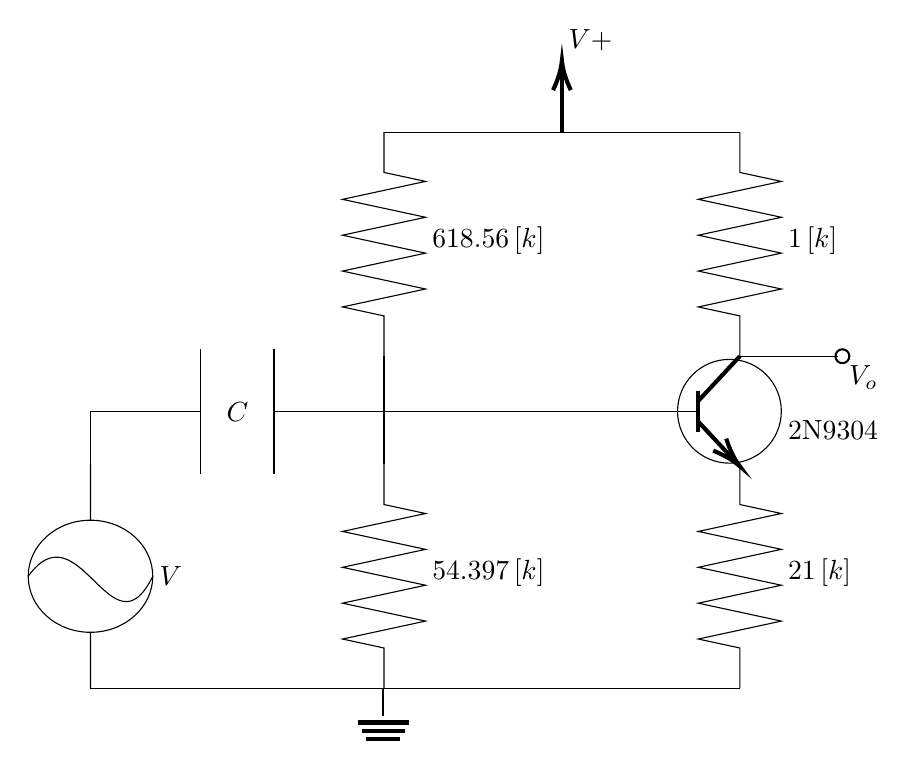
\begin{tikzpicture}[x=0.75pt,y=0.75pt,yscale=-1,xscale=1]
%uncomment if require: \path (0,497); %set diagram left start at 0, and has height of 497

%Shape: Resistor [id:dp08557489822351128] 
\draw   (214,71) -- (214,90.44) -- (234,94.76) -- (194,103.4) -- (234,112.04) -- (194,120.68) -- (234,129.32) -- (194,137.96) -- (234,146.6) -- (194,155.24) -- (214,159.56) -- (214,179) ;
%Shape: Resistor [id:dp5471354453834067] 
\draw   (214,231) -- (214,250.44) -- (234,254.76) -- (194,263.4) -- (234,272.04) -- (194,280.68) -- (234,289.32) -- (194,297.96) -- (234,306.6) -- (194,315.24) -- (214,319.56) -- (214,339) ;
%Straight Lines [id:da10613850567534644] 
\draw    (355.42,205.5) -- (214,205.5) ;
%Shape: Resistor [id:dp42863709400980965] 
\draw   (385.42,71) -- (385.42,90.44) -- (405.42,94.76) -- (365.42,103.4) -- (405.42,112.04) -- (365.42,120.68) -- (405.42,129.32) -- (365.42,137.96) -- (405.42,146.6) -- (365.42,155.24) -- (385.42,159.56) -- (385.42,179) ;
%Shape: Resistor [id:dp18218903209345216] 
\draw   (385.42,231) -- (385.42,250.44) -- (405.42,254.76) -- (365.42,263.4) -- (405.42,272.04) -- (365.42,280.68) -- (405.42,289.32) -- (365.42,297.96) -- (405.42,306.6) -- (365.42,315.24) -- (385.42,319.56) -- (385.42,339) ;
%Shape: Circle [id:dp6263492261348075] 
\draw   (355.42,205.5) .. controls (355.42,191.69) and (366.61,180.5) .. (380.42,180.5) .. controls (394.23,180.5) and (405.42,191.69) .. (405.42,205.5) .. controls (405.42,219.31) and (394.23,230.5) .. (380.42,230.5) .. controls (366.61,230.5) and (355.42,219.31) .. (355.42,205.5) -- cycle ;
%Straight Lines [id:da5434466420085665] 
\draw    (365.42,205.5) -- (355.42,205.5) ;
%Straight Lines [id:da8222789328378522] 
\draw [line width=1.5]    (365.42,215.5) -- (365.42,195.5) ;
%Straight Lines [id:da6868248647799469] 
\draw [line width=1.5]    (365.42,210.5) -- (383.38,229.8) ;
\draw [shift={(385.42,232)}, rotate = 227.07] [color={rgb, 255:red, 0; green, 0; blue, 0 }  ][line width=1.5]    (14.21,-4.28) .. controls (9.04,-1.82) and (4.3,-0.39) .. (0,0) .. controls (4.3,0.39) and (9.04,1.82) .. (14.21,4.28)   ;
%Straight Lines [id:da7170401481045089] 
\draw [line width=1.5]    (385.42,179) -- (365.42,200.5) ;
%Straight Lines [id:da09379764529365986] 
\draw    (385.42,339) -- (214,339) ;
%Straight Lines [id:da37329225941611255] 
\draw    (385.42,71) -- (214,71) ;
%Straight Lines [id:da20374241030260287] 
\draw [line width=1.5]    (299.71,71) -- (299.71,39.58) ;
\draw [shift={(299.71,36.58)}, rotate = 90] [color={rgb, 255:red, 0; green, 0; blue, 0 }  ][line width=1.5]    (14.21,-4.28) .. controls (9.04,-1.82) and (4.3,-0.39) .. (0,0) .. controls (4.3,0.39) and (9.04,1.82) .. (14.21,4.28)   ;
%Straight Lines [id:da7615603326736993] 
\draw    (432.49,179) -- (385.42,179) ;
\draw [shift={(434.84,179)}, rotate = 180] [color={rgb, 255:red, 0; green, 0; blue, 0 }  ][line width=0.75]      (0, 0) circle [x radius= 3.35, y radius= 3.35]   ;
%Straight Lines [id:da09982064594930351] 
\draw [line width=0.75]    (213.71,352.42) -- (213.71,339) ;
%Straight Lines [id:da7825511264162391] 
\draw [line width=1.5]    (201.5,355.42) -- (225.92,355.42) ;
%Straight Lines [id:da8263231613187413] 
\draw [line width=1.5]    (203.5,359.42) -- (223.92,359.42) ;
%Straight Lines [id:da4438946372208784] 
\draw [line width=1.5]    (205.5,363.42) -- (221.92,363.42) ;
%Straight Lines [id:da9620365649992906] 
\draw    (214,339) -- (72.58,339) ;
%Shape: Output [id:dp9760234334247213] 
\draw   (72.58,258) .. controls (89.15,258) and (102.58,270.09) .. (102.58,285) .. controls (102.58,299.91) and (89.15,312) .. (72.58,312) .. controls (56.01,312) and (42.58,299.91) .. (42.58,285) .. controls (42.58,270.09) and (56.01,258) .. (72.58,258) -- cycle (72.58,231) -- (72.58,258) (72.58,339) -- (72.58,312) ;
%Straight Lines [id:da22791584371112872] 
\draw    (72.58,205.5) -- (72.58,232) ;
%Straight Lines [id:da8821366946228647] 
\draw    (214,179) -- (214,205.5) ;
%Shape: Contact [id:dp522587048630987] 
\draw   (99.08,205.5) -- (125.61,205.5) (187.5,205.5) -- (160.97,205.5) (125.61,175.5) -- (125.61,235.5) (160.97,175.5) -- (160.97,235.5) ;
%Straight Lines [id:da5619511756017568] 
\draw    (214,205.5) -- (187.5,205.5) ;
%Straight Lines [id:da6523589746503576] 
\draw    (99.08,205.5) -- (72.58,205.5) ;
%Curve Lines [id:da4854089115611697] 
\draw    (42.58,285) .. controls (67,251) and (83,325) .. (102.58,285) ;
%Straight Lines [id:da7347230772485945] 
\draw    (214,204.5) -- (214,231) ;

% Text Node
\draw (301.71,33.18) node [anchor=south west] [inner sep=0.75pt]    {$V+$};
% Text Node
\draw (436.84,182.4) node [anchor=north west][inner sep=0.75pt]    {$V_{o}$};
% Text Node
\draw (407.42,208.5) node [anchor=north west][inner sep=0.75pt]   [align=left] {2N9304};
% Text Node
\draw (407.42,115.44) node [anchor=north west][inner sep=0.75pt]    {$1\left[\text{k} \si{\ohm}\right]$};
% Text Node
\draw (407.42,275.44) node [anchor=north west][inner sep=0.75pt]    {$21\left[\text{k} \si{\ohm}\right]$};
% Text Node
\draw (236,115.44) node [anchor=north west][inner sep=0.75pt]    {$618.56\left[\text{k} \si{\ohm}\right]$};
% Text Node
\draw (236,275.44) node [anchor=north west][inner sep=0.75pt]    {$54.397\left[\text{k} \si{\ohm}\right]$};
% Text Node
\draw (143.45,205.7) node    {$C$};
% Text Node
\draw (104.58,285) node [anchor=west] [inner sep=0.75pt]    {$V$};


\end{tikzpicture}

      \caption{Final Circuit Design}
      \label{fig:4}
    \end{figure}

\end{enumerate}

\end{document}

